\chead{\textit{Theoretical Approach}}  				
\section{Theoretical Approach}
\label{sec:theo}

This chapter describes all necessary fundamentals to follow along with the mathematical derivation and the implementation in Julia of the decentralized algorithm to solve an optimal power flow optimization problem. First, the economic dispatch process is explained, which is then extended by considering transmission lines and their power flows in the modeling framework. This leads to the concept of optimal power flow optimization. Afterward, the reader is introduced to the \gls{admm} by describing the basics with a simple example. Finally, the current state of research in the context of decentralized algorithms that solve an optimal power flow is summarized.

\subsection{Centralized Economic Dispatch}
\label{sec:theo:ed}

According to \citet{chowdhury1990} and \citet{hetzer2008}, economic dispatch is a technique to allocate all available generators in an electrical power system to minimize the total system costs while making sure that the system load is covered. A concept that is often used to explain the economic dispatch is the merit order curve in which the supply bids of all generators are sorted by their marginal costs in ascending order. These supply bids are accepted as long as the system load is not satisfied. The marginal costs of the last accepted generator define the market price. As a result of this, renewable energy resources are always favored because their marginal costs are insignificant \citep{hetzer2008}. \\

\begin{figure}[h!]
	\centering
	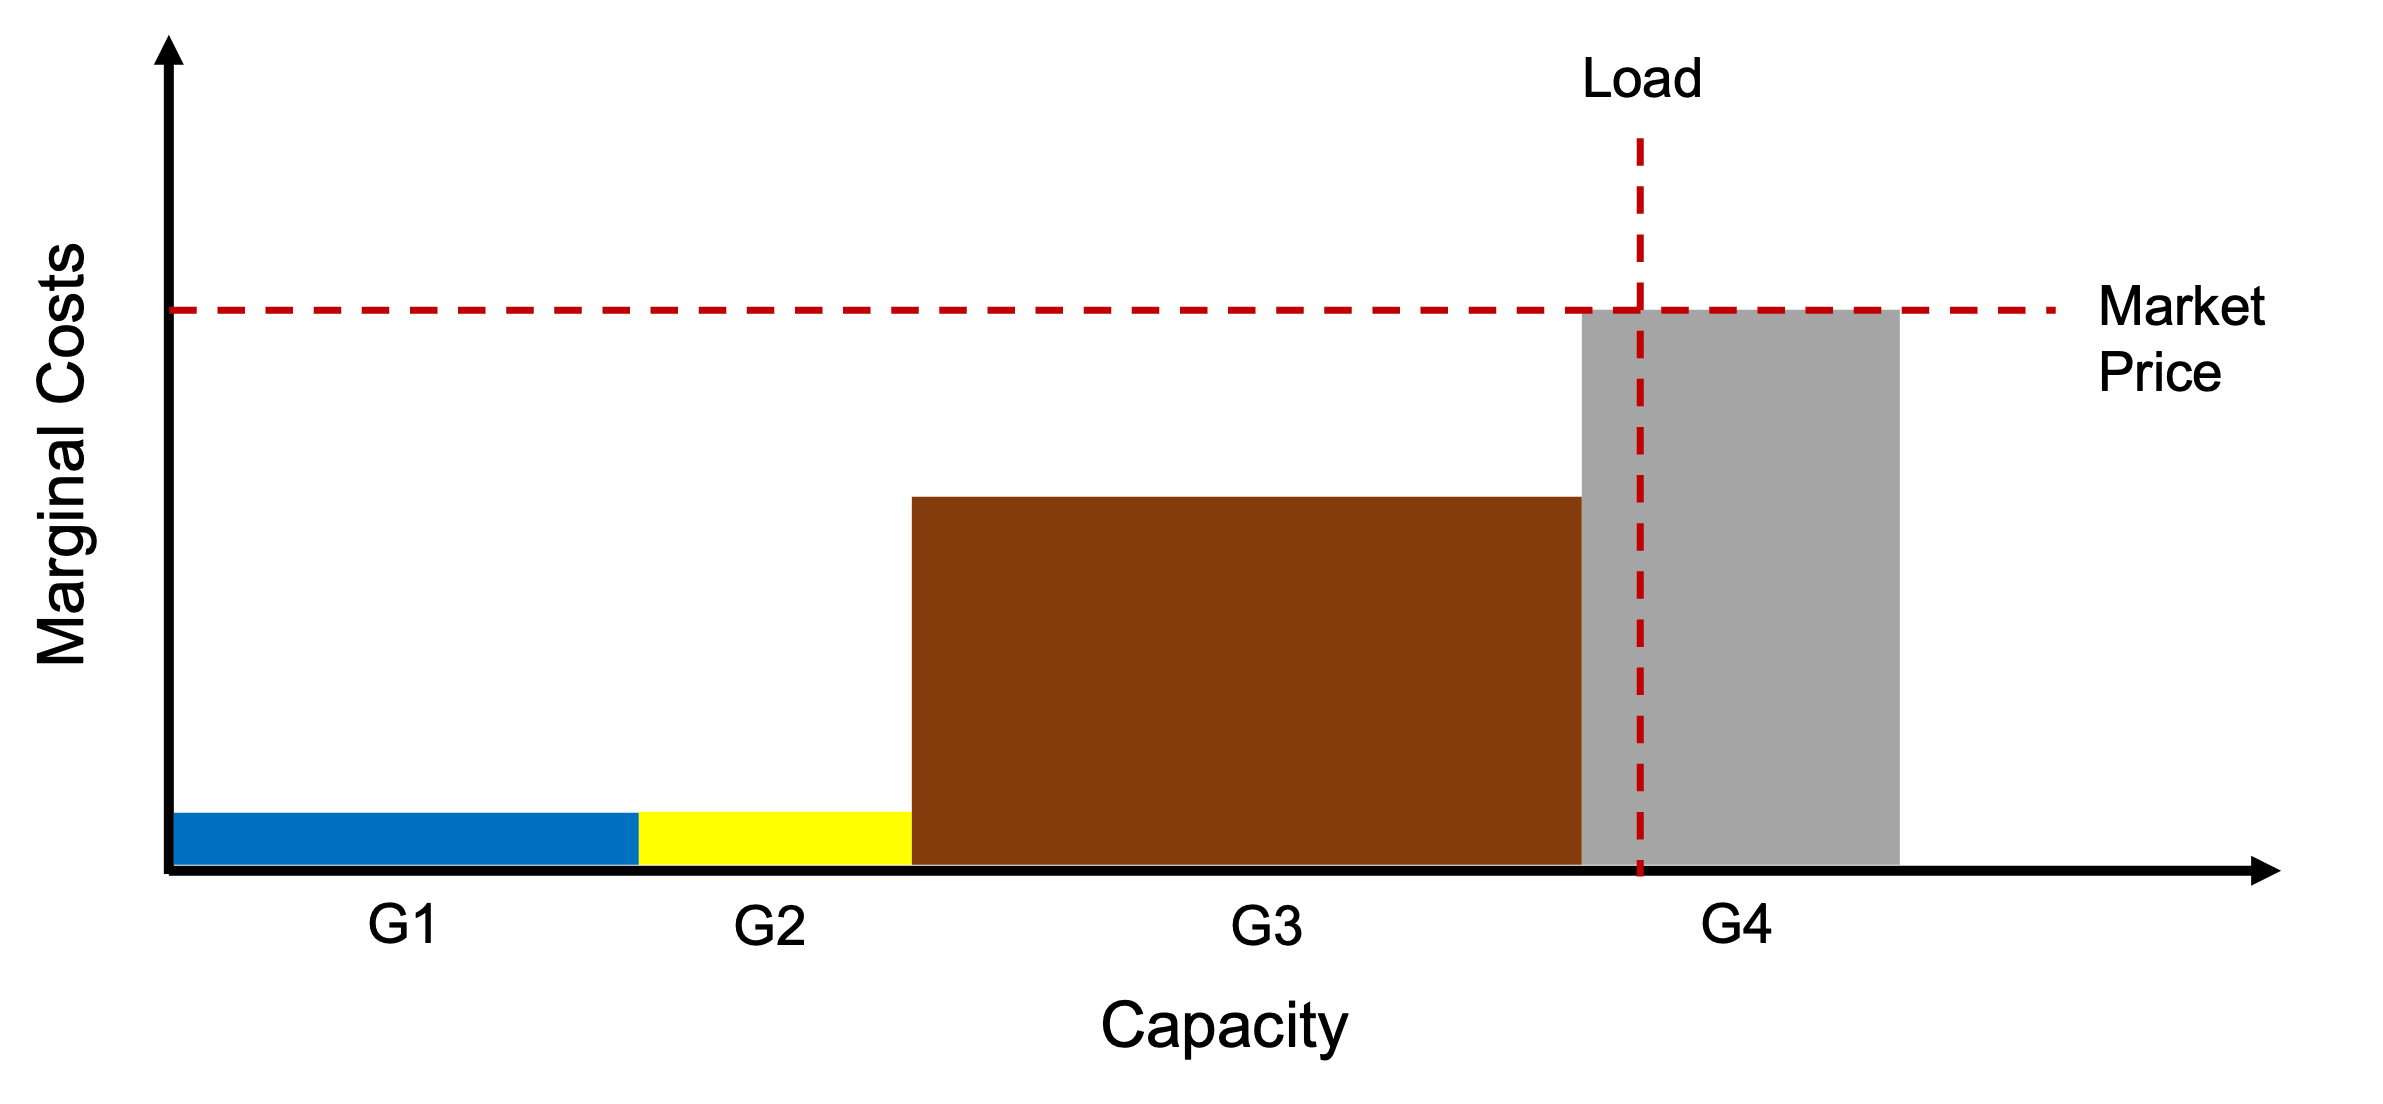
\includegraphics[width=\textwidth]{merit-order-curve.png}
	\caption{Exemplary merit order curve of four generators}
	\label{fig:merit}
\end{figure}

\begin{table}[h!]
    \centering
    \begin{tabular}{lrr}
        Generators $\set{G}$ & $mc$ [EUR/MWh] & $\overline{p}$ [MW] \\ \toprule
        G1 & 0 & 200 \\
        G2 & 0 & 50 \\
        G3 & 30 & 300 \\
        G4 & 50 & 100 \\
        \bottomrule
    \end{tabular}
    \caption{Exemplary generator parameters for an economic dispatch} \label{tab:theo:gen-params}
\end{table}

Figure (\ref{fig:merit}) shows an exemplary merit order curve of four generators out of which two generators, namely generator one (G1) and generator two (G2), are renewable energy resources like photovoltaic or wind. The load is also depicted as a vertical, dashed red line. To solve the economic dispatch, one could use the merit order curve. As figure (\ref{fig:merit}) shows, the capacities of generators one to three are not enough to cover the system load. Thus, generator four must be dispatched, setting the market price to its marginal costs. However, generator four is not producing at its capacity limit. This problem could also be solved by formulating the following cost-minimizing optimization problem:

\begin{subequations}
	\begin{align}
		 \min \quad & \sum_{g\in\mathcal{G}}mc_g \cdot P_{g} \label{eq:theo:ed} \\[10pt]
		 \text{s.t. } \quad & 0 \leq P_{g} \leq \overline{p_g} && \forall g \in \set{G} \label{eq:theo:ed:cap} \\
		 & \sum_{g \in \mathcal{G}} P_{g} = d \label{eq:theo:ed:con}
	\end{align}
\end{subequations}

The above formulation resembles the graphical solution approach of the merit order curve. Equation (\ref{eq:theo:ed}) describes the total system costs that are minimized under two constraints. The power output of the generators has to be within the corresponding capacity limits denoted by constraint (\ref{eq:theo:ed:cap}). Secondly, the demand has to be covered by the production of the generators. This is ensured by constraint (\ref{eq:theo:ed:con}). In comparison to the graphical solution of the merit order curve, this approach has some advantages. First, it can be extended by multiple periods and incorporate further restrictions like ramping constraints. In addition, there exist a lot of algorithms that can quickly solve problem formulations like this, e.g., the simplex algorithm \citep{dantzig1963}. The solution of the cost-minimization for the parameters in table (\ref{tab:theo:gen-params}) and a system load of \SI{560}{\mega\watt} yields total costs of \SI{9500}{EUR} and the following optimal production vector:

\begin{equation}
	P^{\star} = \begin{bmatrix}
		P_{G1}^{\star} \\
		P_{G2}^{\star} \\
		P_{G3}^{\star} \\
		P_{G4}^{\star}
	\end{bmatrix} = \begin{bmatrix}
		200 \\
		50 \\
		300 \\
		10
	\end{bmatrix}
\end{equation}

Based on the findings of \citet{ahlqvist2022} the economic dispatch is a relatively centralized concept because each market participant, e.g., generators in the example above, has to share its detailed cost data and its capacity limits with the intermediary that coordinates the economic dispatch which is in most cases the \gls{tso}. 

\subsection{Centralized Optimal Power Flow}

The problem formulation in equation (\ref{eq:theo:ed}) does not account for any transportation of electricity between locations or nodes in a network. Thus, it would be desirable to include transmission lines into the modeling framework to better simulate electricity transport and, hence, a real-life system. Most of the power systems worldwide rely on power distribution with \gls{ac} \citep{mieth2021}. \gls{ac} is characterized by harmonic functions for voltage and current, resulting in a complex power that is different from the power of a \gls{dc} network. A good explanation of the integration of \gls{ac} into an economic dispatch problem can be found in \citet{weinhold2022}. The subsequent derivation is based on this source.\\ 

Equations (\ref{eq:theo:complex-power}) to (\ref{eq:theo:reactive-power}) describe the complex power $S_n$, the active power $P_n$ and the reactive power $Q_n$ injected at node $n$ for a \gls{ac} system consisting of nodes that are connected by transmission lines.

\begin{subequations}
	\begin{align}
		S_n &= \sum_{k \in \mathcal{N}} V_n V_k(\cos{(\phi_n-\phi_k)} + j\sin{(\phi_n-\phi_k)})(g_{nk} - jb_{nk}) \label{eq:theo:complex-power} \\
		P_n &= \sum_{k \in \mathcal{N}} V_n V_k (g_{nk} \cos{(\phi_n-\phi_k)} + b_{nk}\sin{(\phi_n-\phi_k)}) \\
		Q_n &= \sum_{k \in \mathcal{N}} V_n V_k (g_{nk} \sin{(\phi_n-\phi_k)} + b_{nk} \cos{(\phi_n-\phi_k)}) \label{eq:theo:reactive-power}
	\end{align}
\end{subequations}

Due to the non-linear relation between the variables voltage angle and voltage magnitude, as well as active and reactive power injections at a network node, it is very complicated to integrate these equations in an optimization problem like (\ref{eq:theo:ed}). Fortunately, there are some simplifications for techno-economic studies like this thesis. \citet{vanhertem2006} suggests a linear approximation for the \gls{ac} power flow equations above by applying the following assumptions:

\begin{enumerate}
	\item The voltage angle differences $\phi_n-\phi_k$ are very small resulting in $\sin{(\phi_n-\phi_k)} = \phi_n-\phi_k$ and $\cos{(\phi_n-\phi_k)} = 1$
	\item The resistance of high voltage transmission lines is usually lower than the reactance ($r \ll x$) and can be ignored.
	\item A flat voltage profile ($V_n = 1 p.u.$) exists meaning that all voltage magnitudes are close to their nominal value, e.g. 380 kV.
\end{enumerate}

With these simplifications, it is possible to neglect the reactive power term and simplify the equation for the active power at node $n$ to:

\begin{equation}
	P_n = \sum_{k \in \mathcal{N}} b_{nk}(\phi_n-\phi_k)
\end{equation}

The power flow on a certain transmission line $l$ can be calculated as:

\begin{equation}
	P_l = b_{nk}(\phi_n-\phi_k)
\end{equation}

As explained by \citet{weinhold2022}, these equations are usually written in matrix notation where $\vb{B_d}$ is a diagonal matrix with the line susceptances of each transmission line, $\Phi$ a column vector of nodal voltage angles, and $\vb{A}$ the incidence matrix with dimensions $\mathcal{N} \times \mathcal{L}$ describing the network architecture. In the incidence matrix, a starting node of a transmission line is marked as 1, whereas the end node of a transmission line is characterized by -1. Everything else is zero. The matrix notation then yields:

\begin{subequations}
	\begin{align}
		\vb{P_l} &= \vb{B_d} \cdot \vb{A} \cdot \Phi = \vb{B_d} \cdot \Phi \\
		\vb{P_n} &= \vb{A}^T \vb{B_d} \cdot \vb{A} \cdot \Phi = \vb{B_n} \cdot \Phi \label{eq:theo:nodal-power:matrix}
	\end{align}
\end{subequations}

With the help of the above equations, one can derive a node-to-line sensitivity ($\frac{P_l}{P_n}$) that is also known as the \gls{ptdf}.

\begin{equation}
	PTDF = (\vb{B_d} \cdot \vb{A})(\vb{A}^T \vb{B_d} \cdot \vb{A})^{-1} \label{eq:theo:ptdf}
\end{equation}

Due to the fact that equation (\ref{eq:theo:nodal-power:matrix}) is linear, matrix $\vb{A}^T \vb{B_d} \cdot \vb{A}$ is singular and no inverse can be formulated as required in equation (\ref{eq:theo:ptdf}). A reference node called slack node is introduced to solve this problem that balances all other nodal injections in the network. The slack node is removed from the power flow equations and replaced by zero. The equation for the \gls{ptdf} can be used to calculate the actual power flow on a transmission line $l$ based on the nodal injections $I_n$. The slack node balances all other injections, and the direction of the flow is relative to the signs in the incidence matrix $\vb{A}$.

\begin{equation}
	f = PTDF \cdot I_n \label{eq:theo:flow}
\end{equation}

Equation (\ref{eq:theo:flow}) can be integrated in an economic dispatch while constraining the power flow by the maximum transmission line capacity $\overline{f_l}$. To conclude this section, the example mentioned in section \ref{sec:theo:ed} is extended by an optimal power flow. The generators are allocated at three nodes connected by three transmission lines. The system load is distributed between the nodes. A schema of this network can be found in figure (\ref{fig:opf}). The parameter of the generators are the same as in table (\ref{tab:theo:gen-params}) and the transmission lines are parameterized in table (\ref{tab:theo:line-params}).

\begin{figure}[h]
	\centering
	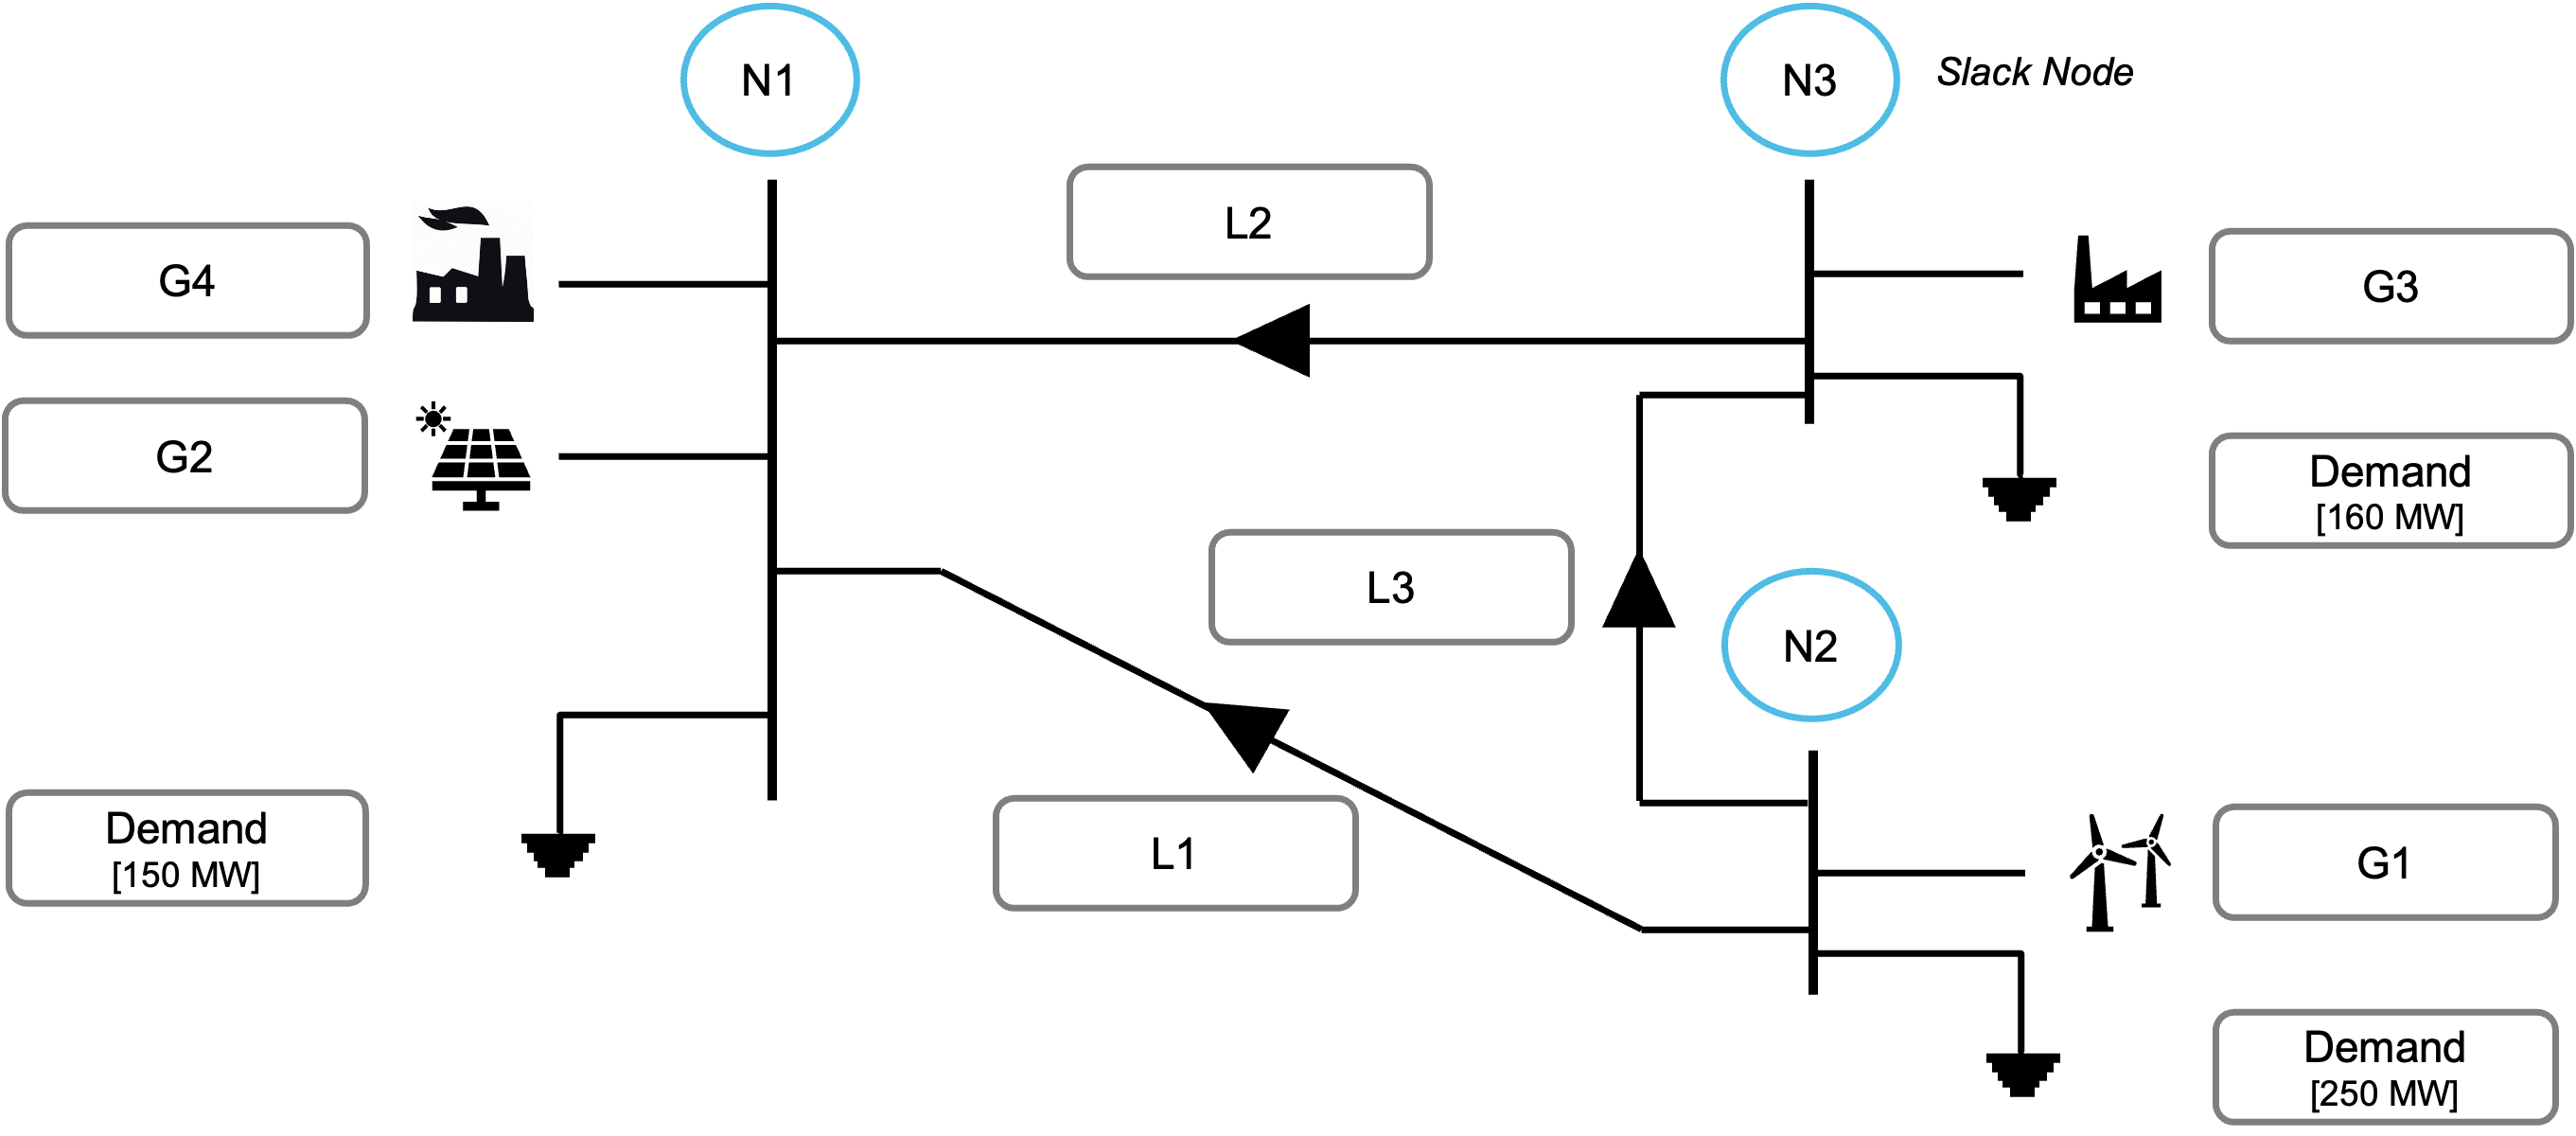
\includegraphics[width=\textwidth]{opf-example.png}
	\caption{Network layout for an exemplary optimal power flow}
	\label{fig:opf}
\end{figure}

\begin{table}[h!]
    \centering
    \begin{tabular}{lccrrc}
        Transmission Lines $\set{L}$ & Start Node & End Node & $S$ [1/$\Omega$] & $\overline{f}$ [MW] \\ \toprule
        L1 & N2 & N1 & 1 & 40 \\
        L2 & N3 & N1 & 1 & 50 \\
        L3 & N2 & N3 & 1 & 100 \\
        \bottomrule
    \end{tabular}
    \caption{Exemplary transmission line parameters for an optimal power flow} \label{tab:theo:line-params}
\end{table}

The optimization problem in (\ref{eq:theo:ed}) has to be extended by an additional constraint to account for the constrained power flows on the transmission lines. The problem formulation for an optimal power flow evolves to:

\begin{subequations}
	\begin{align}
		 \min \quad & \sum_{g\in\mathcal{G}}mc_g \cdot P_{g} \label{eq:theo:opf} \\[10pt]
		 \text{s.t. } \quad & 0 \leq P_{g} \leq \overline{p_g} && \forall g \in \set{G} \\
		 & \sum_{n \in \mathcal{N}} I_n = 0 \label{eq:theo:opf:balance} \\
		 & -\overline{f_l} \leq PTDF_{l,n} \cdot I_n \leq \overline{f_l} && \forall l \in \set{L}, n \in \set{N} \label{eq:theo:opf:flow}
	\end{align}
\end{subequations}

Hereby, equation (\ref{eq:theo:opf:flow}) accounts for the constrained power flows on each transmission line. All power flows have to be within a lower and upper limit that is indicated by the maximum transmission line capacity $\overline{f}$. To calculate the $PTDF$, one needs the susceptance matrix $\vb{B_d}$ and the incidence matrix $\vb{A}$. Based on the example above, these matrices yield:

\begin{equation}
	\vb{A} = \begin{bmatrix}
		-1 & 1 & 0 \\
		-1 & 0 & 1 \\
		0 & -1 & 1
	\end{bmatrix} \quad \quad 
	\vb{B_d} = \begin{bmatrix}
		1 & 0 & 0 \\
		0 & 1 & 0 \\
		0 & 0 & 1
	\end{bmatrix}
\end{equation}


Subsequently, the $PTDF$ can be calculated as:

\begin{equation}
	PTDF = \begin{bmatrix}
		-0.33 & 0.33 & 0 \\
		-0.66 & -0.33 & 0 \\
		0.33 & 0.66 & 0
	\end{bmatrix}
\end{equation}

In addition, constraint (\ref{eq:theo:opf:balance}) makes sure that each nodal demand is still satisfied. The nodal injection $I_n$ used in this constraint is calculated by subtracting the nodal demand from the sum of all of the generators located at that node, see equation (\ref{eq:theo:injection}) for further reference.

\begin{equation}
	I_n = \sum_{g\in\mathcal{G}_n} P_g - d_n
	\label{eq:theo:injection}
\end{equation}

\begin{table}[h!]
    \centering
    \begin{tabular}{lrr}
        Generators $\set{G}$ & Economic Dispatch & Optimal Power Flow \\ \toprule
        G1 & 200 MW & 200 MW \\
        G2 & 50 MW & 50 MW \\
        G3 & 300 MW & 260 MW \\
        G4 & 10 MW & 50 MW \\
        \bottomrule
    \end{tabular}
    \caption{Comparison between generator results of economic dispatch and optimal power flow}
    \label{tab:theo:gen-comparison}
\end{table}

\begin{table}[h!]
    \centering
    \begin{tabular}{lrrr}
        Transmission Lines $\set{L}$ & $\overline{f}$ & Economic Dispatch & Optimal Power Flow \\ \toprule
        L1 & 40 MW & 13.33 MW & 0 MW \\
        L2 & 50 MW & 76.66 MW & 50 MW \\
        L3 & 100 MW & -63.33 MW & 50 MW \\
        \bottomrule
    \end{tabular}
    \caption{Comparison between transmission line results of economic dispatch and optimal power flow}
    \label{tab:theo:line-comparison}
\end{table}

The solution of the optimal power flow problem from equation (\ref{eq:theo:opf}) yields a different generation decision, see table (\ref{tab:theo:gen-comparison}). In comparison to the economic dispatch from section \ref{sec:theo:ed}, generator G4 increases its production from \SI{10}{\mega\watt} to \SI{50}{\mega\watt} while at the same time generator G3 decreases its production from \SI{300}{\mega\watt} to \SI{260}{\mega\watt}. The power output of generators G1 and G2 remains the same. The total costs are \SI{10300}{EUR} and thus \SI{800}{EUR} higher than the economic dispatch due to the higher output of generator G4. The constrained transmission lines explain the difference. As one can see in table (\ref{tab:theo:line-comparison}), the optimal generation vector of the economic dispatch does not consider the maximum capacity of transmission line L2. Since generator G1 already produces at its maximum production capacity, the only way to satisfy the demand at node N1 is to increase the production of the most expensive generator G4. Consequently, generator G3 can decrease its production, resulting in a less utilized transmission line L2. Subsequently, its maximum capacity is ensured. \\

As already written in section \ref{sec:theo:ed}, the economic dispatch is a centralized concept. The same applies to the optimal power flow because there is also one coordinator who has to know the cost details of every market participant, as shown in the example above. 

\subsection{Alternating Direction Method of Multipliers}
\label{sec:theo:admm}

As written in the introduction of this thesis, there is a need to establish new algorithms and procedures to cope with the ongoing transformation of power systems worldwide. Due to the increase of market participants, e.g., installing even more photovoltaic plants, the utilized datasets have become larger and more sophisticated. Subsequently, centralized algorithm schemes will take longer to derive a solution. In this context, the \gls{admm} provides a possibility to create algorithms that are well suited for these large-scale problems incorporating a lot of data points \citep{boyd2010}. The \gls{admm} decomposes the main problem into multiple subproblems. The solutions to the subproblems are then coordinated and combined to derive a global optimum. It combines the methods of Dual Decomposition and \gls{alr}. \citet{boyd2010} provides a thorough explanation and derivation of the \gls{admm} algorithm that was established in the mid-1970-s by Gabay, Mercier, Glowinski, and Marrocco. Another significant advantage of the \gls{admm} is the fact that the algorithm enables decentralization and parallelization by moving from a central problem formulation to several smaller subproblems that can be solved independently. The following section equips the reader with the necessary knowledge about the \gls{admm} to follow along with the thesis.\\

Typically, \gls{admm} solves problems in the form:

\begin{subequations}
	\begin{align}
		\min{(x, z)} \quad & f(x) + g(z) \\
		\text{s.t.} \quad & \vb{A}x + \vb{B}z = c \label{eq:theo:complicating}
	\end{align}
\end{subequations}

Here, $f(x)$ and $g(z)$ are two different subproblems that cannot be solved independently because of the constraint (\ref{eq:theo:complicating}) in which both decision variables are integrated. These constraints are called complicating constraints because they prevent splitting the main problem into multiple, smaller problems. With the help of \gls{alr}, it is possible to remove the complicating constraint and integrate it into the objective function. In comparison to \gls{lr}, \gls{alr} adds a penalty term to the objective function. \gls{alr} is used in the first place because it works for linear as well as quadratic objective functions. See \citet{conejo2006} for further references on \gls{lr} and \gls{alr}. The corresponding Augmented Lagrangian yields

\begin{equation}
	L_p(x,y, \lambda) = f(x) + g(z) + \lambda^T(\vb{A}x + \vb{B}z - c) + \frac{\gamma}{2}\big\| \vb{A}x + \vb{B}z - c \big\|^2_2 \label{eq:theo:al}
\end{equation}

where variable $\lambda$ is the dual variable of the constraint that was relaxed and $\frac{\gamma}{2}\big\| \vb{A}x + \vb{B}z - c \big\|^2_2$ is the penalty term introduced by \gls{alr}. Hereby, $\gamma$ is a damping parameter and the only parameter needed for the \gls{admm}. As for the optimal solution, the penalty term becomes zero. Since the complicating constraint is removed, the function in equation (\ref{eq:theo:al}) could be split. However, the penalty term prevents this due to the second-order norm and the product of the decision variables within. At this point, the \gls{admm} comes into action. It provides a possibility to solve an Augmented Lagrangian by fixing the decision variables to values obtained in the previous iteration of the algorithm. Equation (\ref{eq:theo:al}) can then be transformed and decomposed into two subproblems in which variable $v$ indicates the iteration.

\begin{equation}
	x^{v+1} := \min{(x)} \quad f(x) + g(z^{v}) + (\lambda^v)^T(\vb{A}x + \vb{B}z^v - c) + \frac{\gamma}{2}\big\| \vb{A}x + \vb{B}z^v - c \big\|^2_2 \label{eq:theo:x-update}
\end{equation}

\begin{equation}
	z^{v+1} := \min{(z)} \quad f(x^v) + g(z) + (\lambda^v)^T(\vb{A}x^v + \vb{B}z - c) + \frac{\gamma}{2}\big\| \vb{A}x^v + \vb{B}z - c \big\|^2_2 \label{eq:theo:z-update}
\end{equation}

In equation (\ref{eq:theo:x-update}), decision variable $z$ is fixed and becomes a normal parameter. Thus, the optimal value of $x$ of the next iteration can be obtained by simply solving a minimization problem with one decision variable. The same applies for equation (\ref{eq:theo:z-update}) and decision variable $z$. After solving each subproblem and obtaining the decision variables for the next iteration, the dual variable is updated with the following equation: 

\begin{equation}
	\lambda^{v+1} :=  \lambda^{v} + \gamma(\vb{A}x^{v+1} + \vb{B}z^{v+1} - c)
\end{equation}

As long as the dual variable does not converge, the next iteration is started. The dual variable is converged if the difference between the current and previous value is smaller than a defined threshold. \citet{boyd2010} provide a detailed proof of convergence that will be not covered in this thesis.

\subsection{Current State of Research}

To analyze the current state of research, different literature databases, e.g., IEEE, were searched for studies that investigate a decentralized economic dispatch or a decentralized optimal power flow based on the \gls{admm} algorithm. Two papers that follow a similar approach and methodology as this thesis could be identified. These studies are presented in the following section. \\

\citet{xing2017} study a dynamic economic dispatch problem with energy storage resources in the context of smart grids. They implement an optimization model that includes physical constraints for generators and storages. In addition, they also consider a system spinning reserve. The energy storage resources are included to account for inter-temporal energy arbitrage, reduce the costs of the generators, and improve the spinning reserve. The presented modeling framework does not deal with constrained transmission lines and the corresponding power flows. \citet{xing2017} implement a distributed algorithm based on a consensus-like iterative algorithm and the \gls{admm}. A communication network is established to connect the single elements within the network and enable a decentralized schema. According to the authors of this study, the implemented algorithm is distributed and thus decentralized because no coordinator is needed, and all computation is done locally by the network nodes. The authors evaluate the capability and effectiveness of their algorithm on the IEEE 14-bus network and could determine a convergence after around 15 iterations. Although the mathematical derivation of the distributed algorithm is described in the paper, the study lacks the implementation in any programming language. There is no reference to a published open-source package or a reference to a public repository containing the implementation. \\

The second paper establishes a mathematical framework for a decentralized distribution market that is based on the centralized nodal pricing model \citep{yang2019}. The established market is fully decentralized and does need any coordination from a central entity. The authors use the \gls{admm} to formulate a decentralized algorithm and guarantee the convergence when choosing the correct parameter. Based on the formulation of a centralized market schema, the formulations for a decentralized market are derived. The corresponding mathematical transformations sometimes lack a detailed description, so it is difficult for the reader to follow along. The modeling framework of the study accounts for producers and consumers and power flows on transmission lines. Subsequently, the decentralized distribution market includes an optimal power flow calculation. Since the \gls{admm} can only cope with equality constraints, they transform the inequality power flow constraints into equality constraints by introducing slack variables for the upper and lower power flow capacity limit. However, \citet{yang2019} do not integrate any energy storage resource. Thus, their modeling framework does not reflect current technologies and developments in power systems worldwide. The developed algorithm is tested on a 33-bus and 69-bus system to demonstrate feasibility and efficiency. \citet{yang2019} provide no references to any software implementation of the decentralized distribution market and the related algorithm. \\

Both studies use the \gls{admm} to establish and develop a decentralized algorithm and present a good starting point for decentralized electricity markets. However, none of the studies meets the desired demands. Neither of the studies accounts for both a transmission network and new technologies like energy storage resources. Secondly, the transformation process from a centralized to a decentralized schema is often not explained in great detail. Finally, no study published their software implementation as an open-source package or as a link to a public repository. 
